\documentclass[12pt, a4paper]{article}
\usepackage{caption}
\usepackage{graphicx}
\usepackage{listings}
\usepackage{siunitx}
\usepackage{hyperref}
\def\checkmark{\tikz\fill[scale=0.4](0,.35) -- (.25,0) -- (1,.7) -- (.25,.15) -- cycle;}
\usepackage{tikz-network}
\hypersetup{
    colorlinks,
    citecolor=black,
    filecolor=black,
    linkcolor=black,
    urlcolor=black
}
\usepackage{amsmath, amsfonts, amssymb, amsthm}
\usepackage{algpseudocode}
\usepackage{algorithm}
\renewcommand{\thesubsubsection}{\thesubsection.\alph{subsubsection}}
\title{Algorithms and datastructures\\Exercises}
\date{2022}
\author{Kristoffer Klokker}
\begin{document}
	\maketitle
	\clearpage
	\tableofcontents
	\clearpage
		\setcounter{section}{4}
		\section{Week}
			\subsection{For each function $f(n)$ and time $t$ in the following table, determine the alrgest size $n$ of a problem that can be solved in time $t$, assuming that the algorithm to solve the problem takes $f(n)$ 1 nanosecond}
				\begin{table}[h!]
					\begin{tabular}{|l|l|l|l|l|}
					\hline
							& 1s 			& 1hour			& 1year			& 1 centuray                              	\\ \hline
					$n$    		& $10^9$ 		& $6\cdot 10^{10}$	& $3.2\cdot 10^{16}$	& $3.2\cdot 10^{18}$ 		\\ \hline
					$n \log_2 n$	& $4\cdot 10^7$	& $10^9\frac{1}{\text{s}}\cdot 3600\text{s}=n\cdot \log_2(n)\rightarrow n=  9.8\cdot10^{10}$  & $6.4\cdot 10^{14}$ & $5.6\cdot 10^{16}$                            \\ \hline
					$n^2$      	& $31622$		& $1.8\cdot 10^6$		& $1.7\cdot 10^8$		& $1.8\cdot 10^9$			\\ \hline
					$n^3$       	& $10^3$		& $15326$			& $316010$			& $1.4\cdot 10^6$                       \\ \hline
					$2^n$       	& 30 			& $41.7$			& $54.8$			& $61.5$			           \\ \hline
					\end{tabular}
				\end{table}	
			\subsection{Show that in a puzzle where two peices is switched with $n$ pieces in all wrong positions, it requires at minimum of $n/2$ switches to solve the puzzle}
				For a puzzle with no correct positions in advance, the lowest amounts of move will be in the scenario where every piece's correct position has to piece of its current position. Which therefore will result in $n/2$ amounts of moves is needed.
			\subsection{Create a puzzle with 4 pieces, and find a sequence of switches, but where not every switch moves at least one piece to its correct position}
				\begin{table}[h!]
					\begin{tabular}{|l|l|}
					\hline
					4&1\\\hline
					2&3\\\hline
					\end{tabular}
				\end{table}	
				$4\rightarrow 2,3\rightarrow 2, 1\rightarrow 2$\\
				As seen here this method does no use the greedy method but it still use the same amount of moves.
			\subsection{Create an algorithm which can find cycles in a given puzzle}
				The algorithm takes a list, and creates a variable counter for the amount of cycles.\\
				It then goes through every entry, if the entry is not -1 then it calls a recursive function with the entry index and list.\\
				The list then check if the given entry is -1 if not then set the entry to -1 and then calls itself with the entries last index and the list.\\
				When the function returns it add 1 to the cycle.\\
				Then it returns the amount of cycles\\
				This algorithm will run at $O(2n)$ if the cycle is 1 and it then has to move every entry and go through the rest of the list. 
			\subsection{Use the algorithm implementation to calculate statistic over the amount of cycles in a 16 long permutation}
				\begin{figure}[h!]
					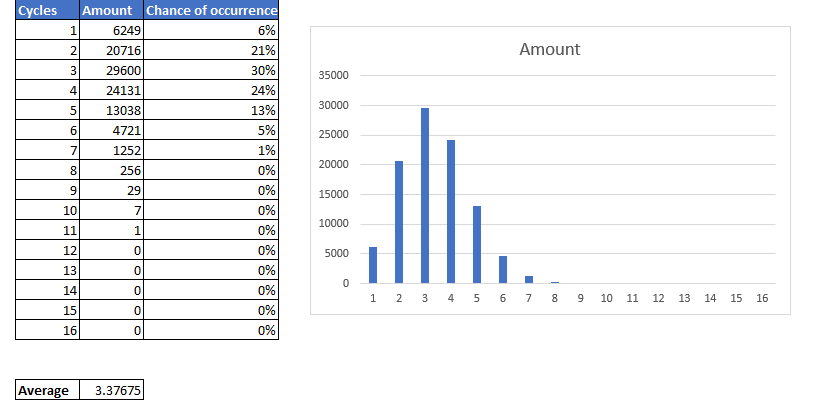
\includegraphics[width=\linewidth]{assets/week5Exercise2.png}
					\caption{Statistic from puzzleSolve/data.csv}
				\end{figure}
			\subsection{Write insertion sort pseudo code}
				\begin{algorithmic}[1]
					\State Linear search($A,v$)
					\State $i=0$
					\While{$i<A.length$ \&\& $A[i]!=v$} 
						\State $i++$
					\EndWhile
					\State return $i$
				\end{algorithmic}
		\section{Week}
			\subsection{What is the average and worst case run time og linear search aglorithm with the element placed randomly}
				Average: on average the run time will be $n/2$ \\
				Worst: if the element is at the end of the list it will be $n$
			\subsection{Let an inversion be that in an array if $i<j$ and $A[i]>A[j]$}
				\subsubsection{Find inversion pairs in $\{2,3,8,6,1\}$}
					$(2,1),(3,1),(8,1),(8,6),(6,1)$
				\subsubsection{For which array will it have the most inverse pairs and how many in an array of length $n$}
					The backwards sorted array, which will have $\frac{n^2-n}{2}$ pairs.
				\subsubsection{What is the relation between inversion pairs and insertion sort}
					The relation is that insertion sort use the same amount of operations in the worst case scenario as inverse pairs.
			\subsection{Analyse the run time of insertion sort, in best case, worst case and random case}
				Here 1000 arrays was used from which random length of arrays was used. Here the are the results of the time divided by length average.\\
				\begin{itemize}
					\item Best - $4.31\cdot 10^{-6}$
					\item Worst - $0.016$
					\item Random - $0.008$
				\end{itemize}
				As seen the random is closest to the worst case. 
			\subsection{Find an algorithm which for a array with integers if there exists a pair which sum is equal to $x$}
				This is done by using a sort like merge sort which takes $n\cdot \log_2n$ then two pointers where one is at the start and one at the end.\\				
				If the two pointers integer sum exceeds $x$ the end moves to the left if less than $x$ the start pointer moves to the right.\\
				This will take $n$ time and therefore the time will still just be $O(n\cdot \log_2n)$
			\subsection{Illustrate merge sort using the array $A=\{3,41,52,26,38,57,9,49\}$}
				\begin{figure}[h!]
					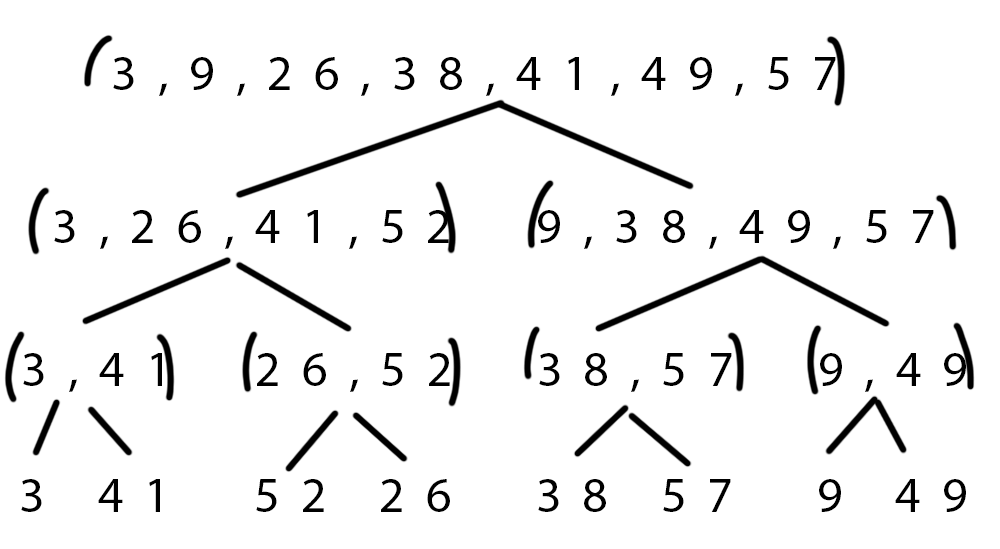
\includegraphics[width=\linewidth]{assets/week6Exercise1.png}
					\caption{Illustration of merge sort}
				\end{figure}
			\subsection{Show that for $f(n)=0.1n^2+5n+25$ that $f(n)=\Theta(n^2)$ and $f(n)=o(n^3)$}
				\begin{align*}
					\lim\limits_{n\rightarrow \infty}\frac{0.1n^2+5n+25}{n^2}=0.1\\
					\lim\limits_{n\rightarrow \infty}\frac{0.1n^2+5n+25}{n^3}=0
				\end{align*}
				Due to the first begin bigger than 0 it means that $f(n)=\Theta(n^2)$ and due to the other being zero means that $f(n)=o(n^3)$
			\subsection{Prove that $max(f(n),g(n))=\Theta(f(n)+g(n))$}
				Due to the max function the highest resullt $g(n)$ can maximally be equal to $f(n)$.\\
				Therefore if $f(n)=n^2$ $g(n)$ can maximally be $n^2$ and therefore the addition will result in the same run time.
			\subsection{Draw binary search, write pseudo code and then code}
				\begin{figure}[h!]
					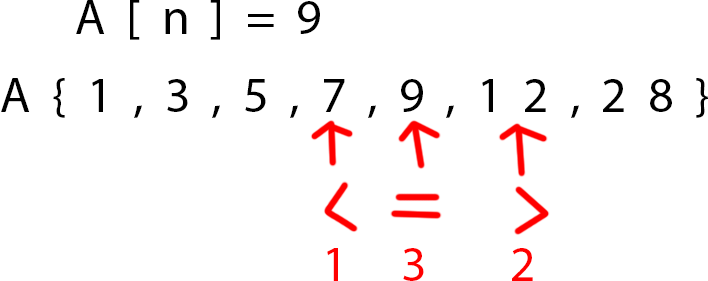
\includegraphics[width=\linewidth]{assets/week6Exercise8.png}
					\caption{Illustration of binary search}
				\end{figure}
				\begin{algorithmic}[1]
					\State Binary search($A,v$)
					\State $i=A.length/2$
					\State $j = A.length/2 + A.length\%2$
					\While{$iA[i]!= v$ $||$ $j==0$} 
						\State $j = j/2 + j\%2$
						\If{$A[i] < v$}
							\State $i = i + j$
						\Else
							\State $i = i - j$
						\EndIf
					\EndWhile
					\State return $i$
				\end{algorithmic}
			\subsection{How can binary search be used to optimize linear search to $O(n\log_2n)$?}
				By instead of linearly going down and finding a number which the current is lower than, a binary search can be done to a number which is lower.\\
				By this every entry will be performed a binary search upon an such the run time will be $n\log_2n$
			\subsection{Is $2^{n+1}=O(2^n)$? Is $2^{2n}=O(2^n)$?}
				$2^{n+1}=2^n\cdot 2^1$ therefore $2^{n+1}=O(2^n)$\\	
				$\lim\limits_{n\rightarrow \infty}\frac{2^n}{2^{2n}}=0$ therefore $2^n=o(2^{2n})$
			\subsection{Prove $\log(n!)=\Theta(n\log n)$}
				$\lim\limits_{n\rightarrow \infty}\frac{\log(n!)}{n\log(n)}=1$ therefore $\log(n!)=\Theta(n\log n)$
			\subsection{Prove $n!=\omega (2^n)$}
				$\lim\limits_{n\rightarrow \infty}\frac{2^n}{n!}=0$ therefore $2^n = o(n!) \rightarrow n!=\omega (2^n)$				
			\subsection{Prove $n!=o(n^n)$}
				$\lim\limits_{n\rightarrow \infty}\frac{n!}{n^n}=0$ therefore $n! = o(n^n) $	
				
					
				
\end{document}


